\chapter{An Issue of Trust}
\label{chap:trust}

Trust and privacy are closely related qualities in
computing~\cite{flowerday2006}. Can we maintain our digital privacy
without having to trust anyone? We can imagine scenarios that maintain
privacy without trust, but they generally involve only storing data on
self-designed, built, and programmed devices that never leave our
possession. Such arrangements are, at best, impractical for the vast
majority of users, and at worst, simply not possible to achieve
today. The range of manufactures, suppliers, and service providers
inherent in the modern computing landscape require that we make
decisions regarding whom to trust at every step of any digital
interaction in which we partake.

The cloud computing model, by its very nature, further amplifies the
number of parties we must trust. But what does it mean to trust a
third party in the cloud? Before discussing the details of an SSaaS
ecosystem, it's helpful to further define ``trust''. In this chapter,
I define a model for analyzing trust and apply this model to compare
various traditional software and technology deployments to SSaaS-backed
options.

\section{Analyses Framework}
\label{chap:trust:framework}

Generally, when we use modern computing devices and services, we must
trust third-party manufactures and service providers with our
data. The manner in which this third party trust relates to the
privacy of user data has two main factors: how much trust do we place
in third parties (e.g. how much of our personal data do we grant them
access to), and in what manner can they violate this trust (e.g. how
can they abuse the access they are granted). I will thus evaluate
computing trust models across two main axes: the \emph{degree} of
trust we must place in third parties, and the manner in which this
trust might be \emph{violated}. Our ideal trust model for a given use
case will minimize the degree of third party trust while also
minimizing the likelihood that such trust will be violated.

In terms of degrees of trust, we can entrust third parties with the
following data-related capabilities:

\begin{packed_desc}
\item[Storage (S):] \hfill \\
  Can a third party faithfully store private user data and make it
  available to the user upon request? Misuse of this capability may
  result in a loss of user data, but won't generally result in the
  exposure of user data.
\item[Access (R):] \hfill \\
  Can a third party read and interpret the private user data they
  store? Misuse of this capability may result in the exposure of user
  data.
\item[Manipulation (W):] \hfill \\ Can a third party modify the
  private user data to which they have access? Misuse of this
  capability may result in the ability to manipulate a user
  (e.g. changing appointments on a user's calendar, etc).
\item[Meta-analysis (M):] \hfill \\
  Can a third party gather user metadata related to any stored private
  user data? Misuse of this capability may result in the ability to
  infer private user data (e.g. who a user is friends with based on
  data sharing patterns).
\end{packed_desc}

I'll define a trust violation as occurring when a third party
exercises any of the above capabilities without explicit user
knowledge and permission. Put another way, a trust violation occurs
whenever a third party leverages a capability with which they are
entrusted in a manner in which the user does not expect the capability
to be leveraged.

I define several types of trust violations based on the manner in
which the violation occurs and the motivations behind it:

\begin{packed_desc}
\item[Implicit (P):] \hfill \\
  This class of trust violation occurs when a third party violates a
  user's trust in a manner approved by the third party. An example
  might be sharing user data with a business partner (e.g. an
  advertiser). Often these forms of violations aren't really
  ``violations'' in the sense that a user may have clicked though a
  Terms of Service agreement that granted implicit permission for such
  use, but if the third party is engaging in behavior that the user
  would not generally expect, an implicit trust violation has
  occurred.
\item[Compelled (C):] \hfill \\
  This class of trust violation occurs when a third party is compelled
  by another actor to violate a user's trust. The most common example
  would be a third party being forced to turn over user data or
  records in response to a request from the government with
  jurisdiction over the party.
\item[Unintentional (U):] \hfill \\
  This form of violation occurs when a third party unintentionally
  discloses or manipulates user data. An example would be a coding
  error that allows either the loss of or unfettered access to user
  data.
\item[Insider (I):] \hfill \\
  This is a subclass of ``Unintentional'' trust violation. This class of
  violation occurs when a privileged adversary within the third party
  violates a user's trust without the permission or knowledge of the
  third party. An example would be a cloud service provider employee
  accessing or disclosing private user data without authorization.
\item[Outsider (O):] \hfill \\
  This is another subclass of ``Unintentional'' trust violation. This
  class of violation occurs when an external adversary gains
  unauthorized access to private user data stored by third party. An
  example would be an adversary exploiting a bug in a third party's
  authorization infrastructure to gain unauthorized access to user
  data.
\end{packed_desc}

\section{Traditional Model}
\label{chap:trust:traditional}

\begin{figure}[t]
  \centering
  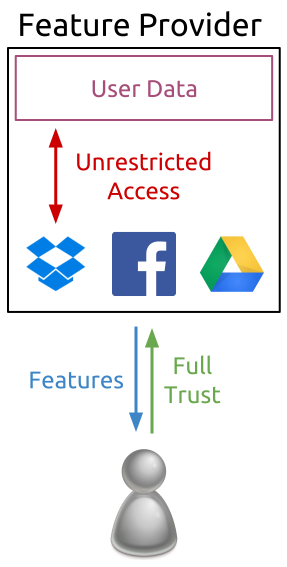
\includegraphics[height=175px]{./figs/out/TrustModel-Traditional.pdf}
  \caption{Traditional Trust Model}
  \label{fig:trust-traditional}
\end{figure}

Existing cloud services are not generally well optimized for
maximizing user privacy. Such services tend to apply an all-or-nothing
trust model where a user must seed a high degree of trust to each
service in order to reap the benefits each service provides. Figure
\ref{fig:trust-traditional} shows the basic trust-for-features
relationship between a user, their private data, and a traditional
cloud service provider.

We can analyze the Dropbox example from \S~\ref{chap:intro:example}
using my proposed framework. To begin, what capabilities is a normal
Dropbox user entrusting to Dropbox? Clearly, users must trust Dropbox
to faithfully store their data since that is Dropbox's core purpose,
so we have granted Dropbox the \emph{S} capability. Furthermore users
must also grant Dropbox the ability to read and access their data
(i.e. the \emph{R} capability) in order to support Dropbox's sharing
and syncing features. While Dropbox doesn't generally utilize it,
users are also effectively granting the manipulation (\emph{W})
capability as well since the user has no mechanisms for ensuring that
Dropbox can't manipulate their data. Finally, Dropbox has full access
to user metadata related to their usage of the service, granting them
the \emph{M} capability. Thus, Dropbox users must trust Dropbox with
all possible capabilities.

But how likely is it that Dropbox might misuse any of these
capabilities, thus violating the user's trust and privacy? In terms of
implicit violations (\emph{I}), Dropbox charges users for storage, and
thus shouldn't generally rely on reading or sharing user data for
advertising purposes. Furthermore, such a business model relies on
Dropbox remaining in its paying users' good graces, disincentivizing
potentially questionable behavior. None the less, there is evidence of
Dropbox opening user files for unknown
reasons~\cite{vintsurf-dropbox}, which might indicate a possible
\emph{I} violation. The user has no way to prevent an \emph{I}
violation when using Dropbox, so we can do no more than give Dropbox
the benefit of the doubt in this area.

In terms of compelled (\emph{C}) violations, Dropbox is a US-based
company, and is thus susceptible to a variety of government-sponsored
data requested, from subpoenas issued under the Third Party
Doctrine~\cite{thompson-thirdparty}, to probable cause search
warrants~\cite{us-constitution-amend4}, to National Security
Letters~\cite{fbi-nsl}, to FISC~\cite{fisc} orders. Dropbox publishes
a transparency report~\cite{dropbox-transparency} indicating how
frequently they are compelled to violate user privacy. Recent versions
of this report indicate that Dropbox receives a few hundred requests
for various user data every 6 months.

Unintentional (\emph{U}), Insider (\emph{I}), or Outsider (\emph{O})
violations are all possibilities when using Dropbox. On the \emph{U}
front, Dropbox had an incident in 2011 that allowed anyone to log into
the service using any password for a 5 hour
period~\cite{dropbox-authbug}. Thus far, Dropbox appears to have
avoided any \emph{I}-type violations, but it has been the target of
various \emph{O}-type attempted violations, primarily built around
advisories who obtain common user
passwords~\cite{dropbox-passwords}. Needless to say, while Dropbox
works to avoid these kinds of violations, they are certainly still
possible, have occurred in the past, and may well occur in the future.

As we can see, a traditional cloud service like Dropbox currently
requires an essentially full degree of user trust (i.e. \emph{S},
\emph{R}, \emph{W}, and \emph{M} capabilities) while also being
susceptible to a full range of trust violations (e.g. \emph{P},
\emph{C}, \emph{U}, \emph{I}, and \emph{O} type violations). Dropbox
is not unique. Other modern computing services from social media
sites, to file lockers, to communication systems all suffer from the
same high-trust, high potential for violations paradigm.

\section{SSaaS Model}
\label{chap:trust:ssaas}

\begin{figure}[t]
  \centering
  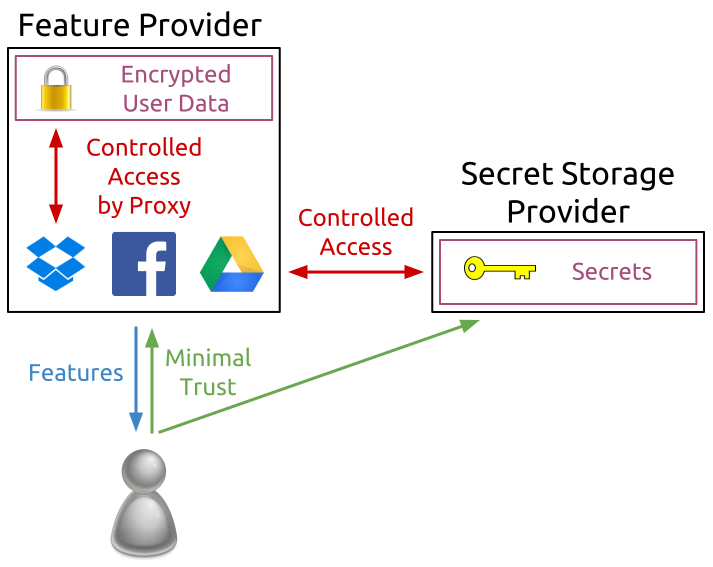
\includegraphics[height=175px]{./figs/out/TrustModel-Seperated.pdf}
  \caption{SSaaS Trust Model}
  \label{fig:trust-ssaas}
\end{figure}

In order to enhance user privacy in the cloud, we must move beyond the
traditional full-trust, easily violated model presented in
\S~\ref{chap:trust:traditional}. Of the two components of my trust
framework, degree of trust and potential for violation, degree is the
easier to control quality: what capabilities to trust a cloud provider
with is largely within the user's control, where as the method in
which trust might be violated is largely outside of a user's
control. I will thus focus my solution on mitigating degree of trust
first while disincentivizing methods of violation second.

The ideal trust model begins with the principle of least
privilege~\cite{saltzer1975}: we should only afford a cloud provider
the minimal degree of trust necessary to provide the intended
features. Furthermore, in order to monitor cloud providers for
potential trust violations, we would also like to maintain some degree
of auditing over any capability we entrust to a provider. Minimal,
audited trust is the basis of my ideal trust model.

Applying this ideal trust model to the previous Dropbox example, I
conclude that Dropbox should really only be afforded the storage
(\emph{S}) capability: after all, there is no real need for Dropbox to
ever be able to access (\emph{R}) or manipulate (\emph{W}) user data
in order to blindly sync files across device or share them with other
users. While Dropbox does not need the metadata (\emph{M}) capability
to simply support the desired user case, it is far more difficult for
the user to limit this capability then the \emph{R} or \emph{W}
capabilities. I thus will also concede this capability to Dropbox as
well. We have thus reduced Dropbox's capabilities from four (full
trust) to two (minimal trust).

But how can we enforce this limited trust profile when using Dropbox?
Figure~\ref{fig:trust-ssaas} shows my proposed SSaaS solution to this
problem. I introduce a new actor: the Secret Storage Provider (SSP)
into the mix. I then restrict the user to only storing encrypted and
authenticated data with Dropbox. The user stores the associated
encryption and verification keys with the SSP. Assuming we utilize
strong encryption and integrity systems like AES~\cite{nist2001} +
CMAC~\cite{dworkin2005}, Dropbox can not feasibly decrypt and access
the user's data nor can they manipulate user data without
detection. Storing the keys with an SSP, as opposed to simply forcing
the user to maintain them manually, has a number of benefits: namely,
it affords users continued support for simple sharing and syncing use
cases. As long as the user's Dropbox client can communicate with the
SSP from any location where they can also communicate with Dropbox,
the user can continue to utilize Dropbox as they traditionally would,
but with significantly less trust in Dropbox itself.

But have we simply replaced one third party with another? Why is the
SSP any more trustworthy than Dropbox itself? There are several reason
why we might expect an SSP to be less prone to trust violations then a
feature provider like Dropbox. I'll discuss these in
\S\ref{chap:ssaas}. But in terms of degrees of trust, we really aren't
affording the SSP any greater degree of trust then Dropbox. Both are
entrusted with the \emph{S} and \emph{M} capabilities, but neither has
the \emph{R} or \emph{W} capability: Dropbox has limited capabilities
because it only holds encrypted and authenticated user data, and the
SSP has limited capabilities because it holds no direct user data at
all, only the cryptographic keys used to protect such data. As long as
the SSP faithfully guards the secret keys they store, the trust model
holds. There are a few new risks in the SSaaS model, however. If both
the feature provider (e.g. Dropbox) and the SSP are located in the
same regulatory jurisdiction, it may still be possible for a single
entity to compel (\emph{C}-type violation) them both or provide data
that would allow an adversary to elevate their capabilities to include
\emph{R} and \emph{W}. Likewise, if Dropbox and the SSP collude to
violate a user's trust, a similar capability elevation will
occur. This latter point introduces a new violation type into my
framework:

\begin{packed_desc}
\item[Colluding (L):] \hfill \\ This class of violation occurs when
  multiple partially-trusted parties collude to gain capabilities over
  user data beyond what the user intended each individually to
  have. An example would be an SSP sharing the user's encryption keys
  with the feature provider storing the corresponding encrypted data.
\end{packed_desc}

This framework provided a basis for analyzing third party trust as
well as the basic argument in favor of SSaaS as a trust-reducing
system. I discuss SSP trust and violation mitigation further in
Chapter~\ref{chap:ssaas}.

\section{Trust Survey of Existing Systems}
\label{chap:trust:survey}

In order to evaluate the trust and security of the SSaaS ecosystem,
it's useful to apply this trust model to a number of existing
scenarios. Each of these applications is discussed in more depth
below.

Table~\ref{tab:trust:app:cap} shows a summery of the capabilities
granted to third parties across a number of common applications. Each
application is rated on a four point scale based on the degree of
trust the application requires the user to place in a third party with
respect to a given capability. ``None'' (zero points) indicates that
the application requires no third-party trust for the given
capability. ``Minimal'' (one point) indicates that indicates that the
application makes concerted efforts to minimize the amount of trust
third parties require, but where some low level of trust may still be
required. ``Partial'' (two points) indicates that the application
takes steps to minimize third party trust for specific capacities, but
still require more trust than is actually necessary. ``Full'' (three
points) indicates that the application does nothing to mitigate third
party trust for a given capability. The score column shows the point
sum of the other columns. Lower scores represent lower degrees of
third party trust.

\begin{table}[!hb]
  \footnotesize
  \centering
  \tabulinesep = 2pt
  \begin{tabu} to \textwidth
    { | X[1,c,m]
      | X[1,c,m]
      | X[1,c,m]
      | X[1,c,m]
      | X[1,c,m]
      | X[0.5,c,m]
      | }
    \hline
    \textbf{Application}
    & \textbf{Storage}
    & \textbf{Access}
    & \textbf{Manipulation}
    & \textbf{Meta-analysis}
    & \textbf{Score}
    \\ \hline
    Dropbox
    & Full
    & Full
    & Full
    & Full
    & 12
    \\ \hline
    Tresorit
    & Full
    & Partial
    & Partial
    & Full
    & 10
    \\ \hline
    Facebook
    & Full
    & Full
    & Full
    & Full
    & 12
    \\ \hline
    Gmail
    & Full
    & Full
    & Full
    & Full
    & 12
    \\ \hline
    PGP/GPG
    & Full
    & None
    & None
    & Full
    & 6
    \\ \hline
    Hangouts
    & Full
    & Full
    & Full
    & Full
    & 12
    \\ \hline
    TextSecure
    & Full
    & None
    & None
    & Minimal
    & 4
    \\ \hline 
    LastPass
    & Full
    & Minimal
    & Full
    & Full
    & 10
    \\ \hline 
    Amazon EC2
    & Full
    & Full
    & Full
    & Full
    & 12
    \\ \hline 
    Single SSP
    & Full
    & Partial
    & Partial
    & Full
    & 10
    \\ \hline 
    Multiple SSPs
    & Partial
    & Minimal
    & Minimal
    & Partial
    & 6
    \\ \hline 
 \end{tabu}
  \caption[Degree of Third Party Trust Across Capabilities]{
    Degree of Third Party Trust Across Capabilities\\
    \textit{[Least Trust] None (0) - Minimal (1) - Partial (2) - Full (3) [Most Trust]}
  }
  \label{tab:trust:app:cap}
\end{table}

Table~\ref{tab:trust:app:threats} shows known and likely trust
violation risk posed by third parties across the same range of
applications. Each application is again rated on a four point scale
based on the likelihood the third party (or parties) providing a
specific application are to commit various types of trust
violations. ``Insider'' and ``Outsider'' type violations are not
included separately since they are really just subclasses of
``Unintentional'' violation. ``Minimized'' (zero points) indicates
that the third parties backing a given application have taken active
steps to minimize the likelihood that a given type of trust violation
might occur (e.g. by publicly fighting court orders, undergoing public
audits and reviews, etc). ``Disincentivized'' (one point) indicates
that the third party's business model or other incentivization factors
actively disfavor a given class of trust violation. ``Vulnerable''
(two points) indicates that a third party has no particular pressure
to avoid committing a certain type of trust violation, but that such
violations have not necessary occurred. ``Known'' (three points)
indicates that a third party has a historic record of committing
specific type of trust violations and has not taken steps to reduce
the risk of such violations in the future. The score column shows the
point sum of the other columns. Lower scores represent less risk of
third party trust violations.

\begin{table}[!hb]
  \footnotesize
  \centering
  \tabulinesep = 2pt
  \begin{tabu} to \textwidth
    { | X[1,c,m]
      | X[1,c,m]
      | X[1,c,m]
      | X[1,c,m]
      | X[1,c,m]
      | X[0.5,c,m]
      | }
    \hline
    \textbf{Application}
    & \textbf{Implicit}
    & \textbf{Compelled}
    & \textbf{Unintended}
    & \textbf{Colluding}
    & \textbf{Score}
    \\ \hline
    Dropbox
    & Disincent.
    & Known
    & Disincent.
    & N/A
    & 5
    \\ \hline
    Tresorit
    & Disincent.
    & Vulnerable
    & Disincent.
    & N/A
    & 4
    \\ \hline
    Facebook
    & Known
    & Known
    & Disincent.
    & N/A
    & 7
    \\ \hline
    Gmail
    & Vulnerable
    & Known
    & Disincent.
    & N/A
    & 6
    \\ \hline
    PGP/GPG
    & Disincent.
    & Disincent.
    & Minimized
    & N/A
    & 2
    \\ \hline
    Hangouts
    & Vulnerable
    & Known
    & Disincent.
    & N/A
    & 6
    \\ \hline
    TextSecure
    & Disincent.
    & Disincent.
    & Minimized
    & N/A
    & 2
    \\ \hline
    LastPass
    & Disincent.
    & Vulnerable
    & Disincent.
    & N/A
    & 4
    \\ \hline
    Amazon EC2
    & Disincent.
    & Known
    & Disincent.
    & N/A
    & 5
    \\ \hline
    Single SSP
    & Disincent.
    & Disincent.
    & Minimized
    & Disincent.
    & 3
    \\ \hline
    Multiple SSPs
    & Disincent.
    & Minimized
    & Minimized
    & Minimized
    & 1
    \\ \hline
  \end{tabu}
  \caption[Risk of Third Party Trust Violations]{
    Risk of Third Party Trust Violations\\
    \textit{[Least Likely] Minimized (0) - Disincentivized (1) -
      Vulnerable (2) - Known (3) [Most Likely]}
  }
  \label{tab:trust:app:threats}
\end{table}

\subsection{Cloud File Storage}

As mentioned, cloud file storage is a popular third party use
case. I've discussed Dropbox~\cite{dropbox} as an example cloud
storage provider extensively in the earlier sections of this
chapter. A summery of the Dropbox trust model results are shown the
Tables~\ref{tab:trust:app:cap} and~\ref{tab:trust:app:threats}. As
previously concluded, Dropbox both requires a full range of trusted
capabilities and is susceptible to (although often disincentivized
from) a range of violations of this trust. Google
Drive~\cite{google-drive}, Microsoft
OneDrive~\cite{microsoft-onedrive}, and related services have similar
trust profiles to Dropbox.

As discussed in Chapter~\ref{chap:related}, a number of systems have
been developed with the aim of overcoming the trust challenges. These
systems include ``end-to-end'' encrypted file storage services such as
Tresorit~\cite{tresorit}. These systems aim to place limits on a third
party's ability to leverage the access (\emph{R}) capability through
the use of client-side encryption. Likewise, they aim to limit third
party access to the manipulation (\emph{W}) capability through the use
of client-side data authentication. In the base case where a user
merely wishes to store data on a single device and not share it with
others, these systems are fairly successful in achieving their desired
trust mitigations. In order to sync data across multiple devices using
such systems, a user must manually provide some secret (e.g. a
password, etc) on each device to bootstrap its operation. While
potentially burdensome and inconvenient, this practice is in line with
these services trusted capabilities mitigation since it does not
require any additional third party trust.

The place where these systems falter at mitigating third party trust
is via their support for multi-user sharing and collaboration. Such
services tend to accomplish multi-user sharing by acting as a trusted
certificate authority (CA) in charge of issuing user
certificates\footnote{A certificate is a combination of a user's
  public key and certain metadata signed by a trusted issuers. See
  Section~\ref{chap:background:crypto} for more information.} These
certificates are then used with various asymmetric cryptographic
primitives (e.g. RSA~\cite{rivest1978}) to exchange the necessary
secrets for bootstrapping sharing between users. Unfortunately, as a
trusted CA, these services are capable of issuing fraudulent user
certificates to themselves or other parties. This allows them to mount
man-in-the-middle (MitM) attacks on any user trying to share data by
impersonating other users utilizing the services. This deficiency is
discussed in depth at~\cite{wilson2014}, and leads to a breakdown of
their claim that their users need not trust third party's, at least
when employing multi-user sharing. By mounting a MitM attack on a user
trying to share data with another user, such service providers can
regain the \emph{R} and \emph{W} capabilities they claim not to
have. Furthermore, these services do little to mitigate their access
to metadata (\emph{M} capability). Nor do they provide ways for users
to avoid data loss in the event that one of the services goes offline
or shuts down (\emph{S} capability).

In terms of trust violations, such ``secure'' cloud storage services
are being paid to store user data, disincentivizing implicit
violations. Compelled violations are possible, although as service
that market themselves as ``privacy'' products, compelled violations
(assuming they are public) are also disincentivized. Due to the CA
trust requirements that exists in such services' sharing
implementations, however, it is possible that such a service could be
compelled to mount a MitM attack on one of their users in order to
provide such data to the compelling party (similar to government
efforts to compel Apple to create a flawed version of OSX that would
be vulnerable to brute force attacks~\cite{ars-cookvfbi}). Similarly,
such a service could be compelled to surrender their CA private key,
allowing the compelling party to take over the trusted CA role and
mount such a MitM attack themselves (similar to the how Lavabit was
compelled to turn over their private TLS keys to facilitate government
access to the data they controlled~\cite{levsion-lavabit}). The fact
that such capabilities have been exploited for the purpose of
committing compelled violations in the past raises the likelihood of
such violations when using services such as Tresorit. Unintentional,
Insider, and Outsider violations are all similar to the traditional
use case: such violations are technically possible, but the third
party at least has a vested interest in avoiding such violations for
reputation-related reasons. Collusion violations aren't really
applicable since Tresorit is a single-party actor.

Furthermore, since services such as Tresorit are not open source or
widely audited by independent parties, the user must trust that the
code they are running to access such services is faithfully
implementing the security guarantees such services claim to
support. It is possible that such a service could ship a flawed
version of their code due to a wide range of trust violations
(e.g. they could be compelled to ship such code, or it could be an
honest unintentional mistake).

A summary of the Tresorit trust model results are shown the
Tables~\ref{tab:trust:app:cap} and~\ref{tab:trust:app:threats}. Such a
service does more to mitigate third party trust and reduce the
likelihood of violations than a traditional cloud storage service, but
still leaves room for improvement. SpiderOak~\cite{spideroak},
Wuala~\cite{wuala}, and related services have similar trust profiles
to Tresorit.

\subsection{Social Media}

Social media sites such as Facebook, Google Plus, etc have become
popular since the early 2000s. Such sites maintain a ``social-graph''
of connections between users, and facilitate communication and sharing
of pictures, events, and other data between users. Such sites are
generally ``free'' to users -- monetizing user data and interactions
for the purpose of selling targeted advertising. Given their ubiquity
in the modern Internet landscape, as well as their position as
ad-suppurated services, it's useful to evaluate modern Social Media
sites using my trust model. Facebook is the largest social media site
today, serving over 1.5 billion users as of 2015~\cite{foster2014}. As
such, I'll evaluate it as an example of the variety of social media
site available today.

In terms of capabilities, Facebook, like Dropbox and other traditional
cloud services, must be trusted with a full range of
capabilities. Facebook is responsible for faithfully storing user
data, Facebook can access and read all data it stores, Facebook can
manipulate the data it stores, and Facebook is capable of performing
meta-analysis of what data users are accessing and of how they are
accessing it.

In terms of likelihood of trust violations, Facebook differs a bit
from cloud-based system like Dropbox in that it is an ad-supported
system. This increases the likelihood of implicit trust failures due
to Facebook's business model being based around the sale of user
data. Indeed, and as mentioned in Chapter~\ref{chap:challenges},
Facebook has a record of implicit trust violations ranging from the
Emotional Contagion Study~\cite{goel2014} to its use of user's photos
in the ads it serves~\cite{mashable-socialads}. Beyond implicit trust
violations, Facebook's trust violation profile is again similar to
other traditional cloud services such as Dropbox. Like
Dropbox~\cite{dropbox-transparency}, compelled violations are known to
occur~\cite{facebook-transparency}. Unintentional, insider, and
outsider violations are all possible, but Facebook has an active
interest in avoiding them. Collusion violations aren't really
applicable since Facebook is a single-party actor.

Tables~\ref{tab:trust:app:cap} and~\ref{tab:trust:app:threats} show a
summery of the Facebook trust model analysis. Google
Plus~\cite{google-plus} and related social-media services have similar
trust profiles to Facebook.

\subsection{Communications}

Communication systems ranging from email and chat to voice and video
calling are another popular modern use case. The privacy and security
of these systems are a matter of great public concern, and indeed many
of the current legal privacy and security battles revolve around the
ability to communicates in a private and secure manner
(e.g.~\cite{apple-fbiletter, greenwald-prism, levsion-lavabit}). It is
thus useful to apply my trust model to the analysis of several such
services. I'll analyze both traditional (Gmail) and secure (GPG/PGP)
email services as well as traditional (Google Hangouts) and secure
(TextSecure) chat/messaging
applications. Tables~\ref{tab:trust:app:cap}
and~\ref{tab:trust:app:threats} show a summery of these analyses.

Gmail~\cite{google-gmail} and Hangouts~\cite{google-hangouts} are both
Google-hosted communication services - placing them fairly soundly in
the ``traditional cloud services'' camp. As such, their profiles are
similar to those of Dropbox and Facebook. Both services require
granting Google a full range of capabilities over user data.

Like Facebook, both services are ad-supported - increasing the
likelihood of implicit trust violations (although unlike Facebook,
Google seems to have a better track record of not committing such
violations). Similarly, both services are known to be subject to
compelled violations~\cite{google-transparency}\footnote{It's possible
  such cloud communication services are actually at an increased risk
  of compelled violations relative to other cloud services due to the
  existence of laws such as the Communications Assistance for Law
  Enforcement Act (CALEA)~\cite{calea-usc, calea-fcc} specifically
  designed to aid the government in obtaining a user's
  communications.}, and are disincentivized, although by no means
immune, from committing unintentional, insider, and outsider
violations\footnote{Google has taken steps to ensure communication
  between all of its data centers and between mail servers are
  encrypted in transit, helping to minimize outsider
  violations~\cite{gmail-blog-encryption}. Similarly, it has recently
  started providing end users with information as to whether or not
  encrypted email transmission was possible and whether or not an
  email's sender has been authenticated~\cite{gmail-blog-indicators}.
  In both cases however, third parties, not end users, remain in full
  control of all the necessary encryption keys, limiting this
  protection to the mitigation of outsider violations, and doing
  little to mitigate implicit, compelled, unintentional, or insider
  violations.}. Thus, Google is able to analyze, alter, and expose any
data that travels across its network using either service - either of
it's own volition or due to a compelled order or unauthorized data
breach.

The OpenPGP protocol~\cite{callas2007} is one of the traditional
mechanisms for securing digital communications. It is most widely used
with email - and is implemented in a wide variety of applications from
desktop apps such as GnuPG (GPG)~\cite{gnupg} to browser-based plugins
such as Mailvelope\cite{mailvelope}. The OpenPGP protocol utilizes
public-key cryptography to end-to-end encrypt and authenticate
messages traveling across untrusted mediums. It can be applied atop
mail traversing traditional email systems such as Gmail as well as to
messages traversing chat applications such as Google Hangouts. When
used with such service, PGP provides an additional level of trust
mitigation above and beyond what is possible to achieve via the native
services themselves. In terms of trusted capabilities, a user
employing PGP atop a traditional third party cloud service such as
Gmail minimizes both the third party's access (via encryption) and
manipulation (via authentication) capabilities. In such a scenario
only the end-users involved in a given communication, and not any
third party through which that communication might pass, have access
to the necessary cryptographic keys required to read or alter the
message. The third party, however, can still capture metadata about
the communication since such metadata is outside of the scope of the
message content that PGP is capable of securing. The third party is
also still capable of dropping or deleting the communication all
together, and thus still poses the ``storage'' capability.

Since the OpenPGP protocol and associated implementations are not
controlled by any single third party, there is no straightforward
analysis of its likelihood of PGP-related trust violations. In
general, however, PGP implementations are controlled by parties with a
vested interest in maintaining user security and privacy. Thus such
parties are strongly disincentivized from committing implicit or
compelled violations. Most OpenPGP implementations are also open
source. This helps to mitigate\footnote{Although it does not
  necessarily prevent such violations.  E.g. as in
  Heartbleed~\cite{heartbleed} or a Ken Thompson style
  attack~\cite{thompson1984}.} unintentional, insider, and outsider
violations by maximizing the number of eyes on the code and reducing
the likelihood of mistakes or intentionally coded vulnerabilities and
back doors.

Due to the numerous challenges and deficiencies associated with using
OpenPGP-based systems~\cite{green-pgp}, developers have created a
number of alternate secure communication protocols. These protocols
aim to provide forward-secrecy, metadata privacy, deniability, contact
authentication, and message encryption and authentication for
(primarily) real-time communication such as instant messaging and chat
systems. Examples of such protocol include OTR~\cite{otr-v3} and
OTR-derived protocols like TextSecure~\cite{otr-advanced-ratchet}. The
TextSecure protocol is used by several apps such Open Whisper System's
Signal~\cite{openwhisper} and WhatsApp~\cite{whatsapp}. TextSecure is
thus a useful target to analyze under my trust framework.

TextSecure is an OTR-derived asynchronous secure messaging
protocol. It uses various forms of asymmetric cryptography to provide
users with end-to-end encrypted and authenticated individual and group
messaging capabilities. TextSecure has been formally analyzed and
proven to provide secure encryption and message
authentication~\cite{frosch2014}. Use of TextSecure thus denies any
third party through which TextSecure message might pass (including the
TextSecure server itself) the access or manipulation
capabilities. Furthermore, TextSecure makes efforts to secure all
metadata from non-participating actors as the server itself. This
strongly curtails a third party's ability to analyze message
metadata. It is still possible for a network-level adversary or the
TextSecure server to discover the raw network (e.g. IP) endpoints
involved in a TextSecure exchange, but higher level details are not
available. It's also possible to couple TextSecure with existing
network anonymity systems such as Tor to mitigate such network-level
meta-analysis~\cite{intercept-chatting}. TextSecure users are still
dependent on a third party to operate a TextSecure server in order to
communicate in the first place (e.g. it's not a fully distributed
protocol), but beyond this ``storage''-like capability, TextSecure
grants no other capabilities to any third party.

Like OpenPGP, TextSecure is a protocol implemented by several
different apps. Such application providers (e.g. Open Whisper Systems)
specifically market their products as being a secure alternative to
more traditional chat systems, and thus are strongly dissuaded from
committing any kind of implicit or compelled trust
violation. Furthermore, most TextSecure implications are open source,
which mitigates the likelihood of unintentional\footnote{Researchers
  have discovered bugs in TextSecure, but these bugs were quickly
  patched~\cite{frosch2014}.}, insider, or outsider
violations. TextSecure has also undergone external audits and reviews,
further decreasing the likelihood of an unintentional or insider
violation~\cite{frosch2014}. As in OpenPGP, even if a violation
occurred, the capability restrictions discussed above severely limit
what data the violation would expose. TextSecure thus represents a
successful effort to reduce third party trust exposure and secure user
communications.

\subsection{Password Managers}

Probably the most common variant of a ``secret storage'' system is
manifest by consumer-oriented password management programs. Such
programs are useful for helping end-users remember passwords, and by
extension, for encouraging users to use stronger (i.e. longer and/or
more random) passwords~\cite{brodkin-passman, krebs-passwords,
  schneier-passwords}. It's thus useful to evaluate the trust model
surrounding such programs. LastPass~\cite{lastpass} is one of the most
popular cloud-based password managers. I'll thus apply my trust model
to a typical LastPass deployment. The results are summarized in
Tables~\ref{tab:trust:app:cap} and~\ref{tab:trust:app:threats}.

LastPass operates by storing encrypted user passwords on a
LastPass-controlled server. Passwords are encrypted on the client and
only encrypted passwords are sent to LastPass. Each password is
encrypted using a key derived from a user-supplied ``master''
password. LastPass never stores this master password directly, making
it difficult for them to derive the key necessary to decrypt the
encrypted data they store. Thus, LastPass limits it's ``access'' to
user data. LastPass does not, however, appear to perform any kind of
cryptographic authentication on the data it stores, meaning it still
has full capabilities over the ``manipulation''
capability.\footnote{In realty, it is somewhat difficult for LastPass
  to modify user data intelligently since they lack the ability to
  read the result of their modifications. Nonetheless, the lack of any
  client-side cryptographic protections against modification leaves
  the door open to a range of potential attack on LastPass's client
  side encryption, as per the ``cryptographic doom''
  principle~\cite{marlinspike-doom}.}  Similarly, LastPass is fully
responsible for faithfully storing user data and has full access to
all user metadata associated with any stored password.

In terms of likelihood of trust violations, LastPass has a very
similar profile to a service like Tresorit. LastPass is a ``freemium''
service that generates its income off its ability to faithfully store
and protect user passwords. This disincentivizes implicit trust
violations. LastPass also has a strong incentive to minimize (at least
public) compelled violations, although it is still subject to such
violations. Unintentional, insider, and outsider violations are
similarly disincentivized, although they have occurred
before~\cite{lastpass-blog-breach}.

Like Tresorit, LastPass is not open source nor subject to public code
audits. As such, the user is required to trust the LastPass has
faithfully coded it's software not to expose additional capabilities
via hidden back doors. It is thus possible that LastPass could be
compelled to modify the LastPass client program to do something like
send copies of a user's master password back to LastPass where it
could be used to decrypt all of the user's data. It's also possible that
the lack of cryptographic authentication on user data would allow
LastPass to mount a range of attacks on a user - potentially revealing
one or more of the passwords they store with LastPass in the process.

\subsection{Cloud Infrastructure Services}

Most modern cloud services are operated atop infrastructure provided
by shared infrastructure service provides such as Amazon or
Google. The benefits of such arrangements are discussed in detail in
Section~\ref{chap:background:cloud}. Given that cloud infrastructure
is the primary method of deploying most modern software, it's useful
to analyze the trust a user of such a service must place in their
provider. I'll analyze Amazon's Elastic Cloud Compute (EC2) service as
a typical Infrastructure-as-a-Service (IaaS) example. A summery of the
results appears in Tables~\ref{tab:trust:app:cap}
and~\ref{tab:trust:app:threats}.

Amazon EC2~\cite{amazon-ec2} allows user to spin up virtual machines
(VMs) running user-specified operating systems and code atop
Amazon-owner servers. In such a situation, a user can control the
specification of their VM, but are entirely reliant on Amazon to
faithfully provide the underlying hardware. The traditional wisdom in
computer security is that anyone who controls the hardware has the
ability to subvert any software-level security control implemented
atop it. Thus, since Amazon controls the hardware underlying EC2, they
effectively have full control over any data end-user store atop
EC2. Amazon could (theoretically) read all a VMs memory or disks, or
even alter the behavior of the processor in such a system to control
the execution flow of any software running atop it. EC2 thus requires
the end user to grant Amazon full capabilities to store, read, modify,
or meta-analyses any the data stored or processed via an EC2-backed
VM\footnote{It is potentially possible to use encryption system that
  don't require ever storing the encryption key itself atop
  Amazon-controlled infrastructure to work around some of these
  issues, but such systems are beyond the standard EC2 usage base case
  discussed here.}.

The profile of Amazon's proclivity for trust violation follow that of
other service-oriented cloud operators such as Dropbox, LastPass,
etc. Amazon charges users for the right to use EC2, and faces
competition from numerous other actors in the cloud service provider
space. Thus, Amazon is strongly disincentivized from committing any
form of implicit trust violations. Amazon, like other third parties,
is subject to a range of compelled
violations~\cite{amazon-transparency}. Likewise, Amazon is
disincentivized, but not immune ti, unintentional insider or outsider
violations.

\subsection{SSaaS Alternatives}

All of the applications analyzed thus far have employed various
non-SSaaS-based models for security and secret management. For
comparison, I present an analysis of the two primary Secret Storage as
a Service models discussed in Chapter~\ref{chap:ssaas}: a single
secret store provider (SSP) model and the multi storage provider
model.

In the single SSP model, the end user store their secrets with a
single SSP third party, potentially using these secrets to protect a
separate set of data stored with traditional cloud provider. Such a
model is used by the Custos prototype presented in
Chapter~\ref{chap:custos} as well as existing secret storage systems
such as Hachicorp's Vault~\cite{vault}. In such a model, the end user
is still grating one or more third parties the full ``storage''
capability since the failure of other the SSP or the traditional cloud
provider will result in a loss of user access top their data. In such
a scenario, however, the end user is granting a more limited set of
``access'' and ``manipulation'' capabilities since no single third
party has access to both the users data and the secrets necessary to
decrypt or alter it. E.g. the user can store encrypted and
cryptographically authenticate data atop Dropbox and store the
associated crypto keys with their SSP, ensuring that neither the SSP
nor Dropbox can easily read or manipulate their data. The SSP can,
however, modify and read the user's secrets themselves, which
depending on the use case, may still allow them to access a variety of
user data depending on the nature of the SSP-backed application in
question. Similar to previously discussed systems, the single-SSP
model still allows both the SSP and any associated cloud storage
providers a high degree of access to user metadata regarding the
secrets they store or the data such secrets exist to protect.

In terms of likelihood of trust violations, the single-SSP model is
similar to other privacy-preserving applications such as
TextSecure. In an SSaaS ecosystem, there should be a multitude of
competing SSPs, one or more of which an end-user will pay for secret
storage. Such competition coupled with the storage-for-profit business
case strongly disincentivizes both implicit trust failures by any
single SSP. Compelled violations are similarly disincentivized - and
it is likely that an SSP would take steps to minimize compelled
failures in order to uphold it's reputation. Unintended violations can
also be mitigated by ensuring SSPs use publicly audited and/or open
source implementation of their systems. A single SSPs is, however, at
risk of colluding with whichever cloud provider a user is using to
store the corresponding encrypted data for the keys they store with
their SSP. If such an SSP colluded with such a storage provider, both
parties could succeed in accessing the user's data and regaining the
``access'' and ``manipulation'' capabilities they claim to avoid.

In order to improve upon the trust degree and risk inherent in the
single-SSP model, it's possible for user to move to a multi-SSP SSaaS
model. In such a model, the user shards their secrets across multiple
SSPs using a $n$ choose $k$ scheme the provided both privacy and
redundancy (details of such schemes are discussed in more depth in
Section~\ref{chap:ssaas:trust}). The multi-SSP model provides a
reduced degree of trust profile compared to the single-SSP model. In
such a scenario, the user can mitigate the need to trust any single
third party with the ``storage'' capability since they have now
redundancy spread their data across multiple SSPs. Thus the failure of
a single (and potentially more, depending on the values of $n$ and
$k$) SSP will not result in data loss. Furthermore, the ``access'' and
``manipulation'' capabilities are further reduced since no single SSP
has access to the user's secrets. Furthermore, the use of
multiple-SSPs may even reduce the user's metadata exposure by allowing
the user to reduce having any single SSP hold all of their secrets or
see all of their secret access patterns.

The multi-SSP model also reduce the risk profile associated with SSP
trust violations. As in the single-SSP use case, implicit violations
are disincentivized by nature of the SSP business model. In the
multi-SSP use case, however, compelled violations are further
minimized since no single SSP can be compelled to provide all of the
require data to access a user's secrets. As such, a compelling entity
would be forced to compel multiple parties, potentially located across
multiple jurisdictions, in order to access a user's
secrets. Unintended violations are again minimized assuming prudent
use of open source code and public audits. The risk of
collusion-related violation are also further reduced due to the fact
that the multi-SSP use case requires a greater number of colluding
parties to succeed in mounting a collusion-type violation. The greater
the number of required colluding parties, the less likely such a
collusion is to occur.

Tables~\ref{tab:trust:app:cap} and~\ref{tab:trust:app:threats} provide
a summer of both the single-SSP and multi-SSP SSaaS models. As these
tables show, the trust profiles of such models score on par or better
than existing privacy-enhancing systems such as PGP and Tresorit. As
discussed in other chapters, however, such models offer additional
functionality above and beyond that achievable using more traditional
solutions.

%%  LocalWords:  SSaaS FISC SSP CMAC OneDrive Tresorit Disincent MitM
%%  LocalWords:  SpiderOak Wuala Lavabit LastPass CALEA
%%  LocalWords:  Mailvelope TextSecure OTR WhatsApp LastPass's IaaS
%%  LocalWords:  freemium SSPs Heartbleed Custos Hachicorp's
